\chapter{结\texorpdfstring{\quad}{}论}

本文基于Python的开源硬件生成框架PyHCL,实现了面向DSP的基于RISC-V指令集的RV32GCP嵌入式微处理器内核以及SoC片上系统。本文所实现的微处理器为4级单发射顺序执行流水线结构,实现了RISC-V基本32位整数指令集“I”、乘除指令集“M”、压缩指令集“C”、单精度与双精度浮点指令集“F”与“D”、原子操作指令集“A”以及针对低功耗的SIMD扩展指令集”P“。微处理器实现为4级单发射顺序执行流水线结构,实现了机器特权级模式以及CLINT中断控制器,支持软件中断嵌套。在保持低资源占用的同时,性能与ARM Cortex-M3基本持平。本文所实现的微处理器能够填补目前开源低功耗嵌入式RISC-V微处理器实现的空缺。

而实现本文微处理器RTL级电路描述的开源硬件生成框架PyHCL,是基于Python的集电路设计与验证一体的硬件全栈开发框架,PyHCL使用标准PyHCL原语的方式构建RTL级电路逻辑,包含有完整的中间语法树以及FIRRTL后端生成器。此外,PyHCL还提供了多种验证测试方法,并基于本文实现的RV32GCP微处理器内核开发了基于混合仿真方法的多级验证测试平台,针对RISC-V微处理器内核开发了对应的差分测试框架。通过PyHCL以及本文所实现的微处理器,可以探索到硬件敏捷设计模式的冰山一角。如图5-1所示,是结合PyHCL开发本微处理器的FPGA原型的流程。总体开发的流程从给定微处理器内核的系统规格开始,在这一步会给出微处理器内核所要实现的基本特性,同时在这一步也会进行验证环境的开发。当进入电路设计阶段时,验证的工作也会同时开始。整个处理器核包含多个开发周期,从最开始实现的基本RV32IMC软核,再逐一添加浮点支持、原子操作以及“P”扩展指令功能。每个开发周期都包含有若干功能的实现,对应若干模块的RTL级实现以及验证。在模块级的设计与验证当中,使用PyHCL的RTL级实现与模块级单元测试交织进行,验证策略使用多级验证环境中提供的PyHCL-Tester+Treadle。当前迭代开发周期中的功能实现后,进入整个微处理器系统的集成测试阶段,多级验证环境中可以根据当前验证需要配置不同的验证构件参数而不需要重新设计,来适配不同功能模块的集成测试流程。通过结合PyUVM以及PyHCL-Tester的验证方法,可以保证性能的同时提供一定的可重用性以及稳定性。系统验证后的Verilog代码将会在EDA工具中进行综合与实现,并最终生成FPGA比特流写入到开发板上进行测试,至此一个开发周期完成。

\begin{figure}[htbp]
	\centering
	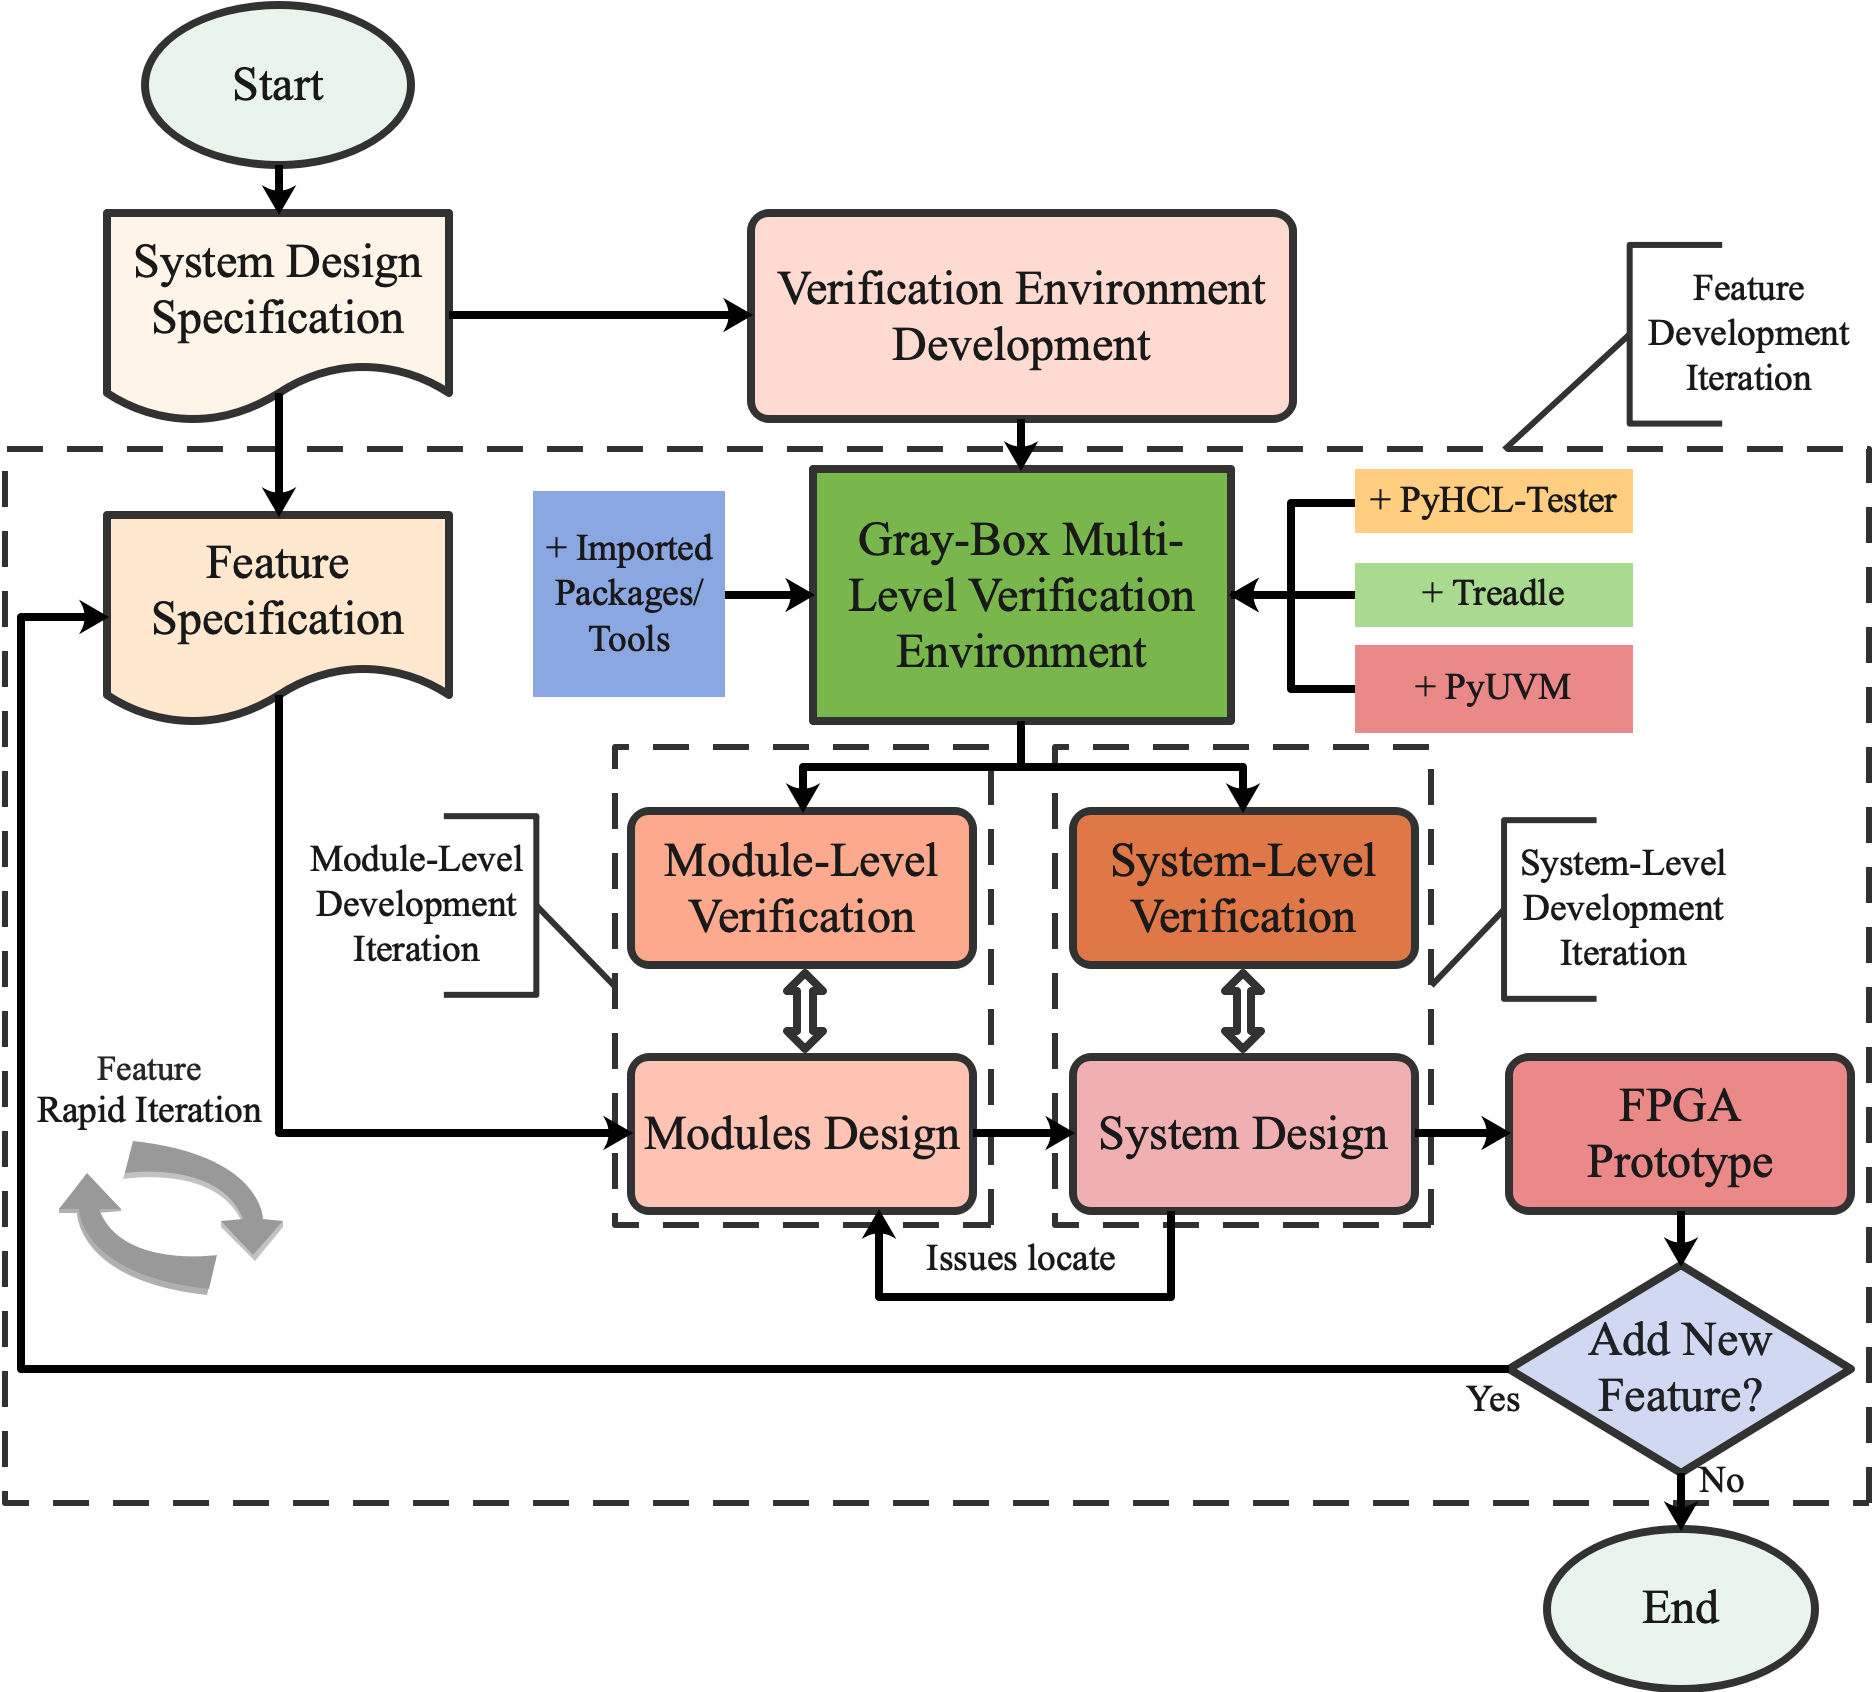
\includegraphics[width=0.95\textwidth]{Photos/process.png}
	\caption{基于PyHCL开发本文实现的RV32GCP微处理器内核FPGA原型的开发流程}
\end{figure}

在微处理器内核每个功能的开发周期当中,设计与验证时交织在一起进行的,而不是当设计全部完成后再进行验证,这可以大大缩短每个开发周期的时间,快速迭代完成FPGA原型开发并上板验证,以此来达到硬件敏捷设计的效果。在未来,PyHCL将会继续探究基于ASIC为后端的开发,并将本文所实现的RV32GCP内核完成ASIC后端的特定工艺流程。

综合全文的内容,本文所做的研究工作总结如下:

\begin{enumerate}
	\item 本文实现了基于RISC-V的RV32GCP微处理器内核,微处理器实现了基于“P”扩展指令集的低功耗SIMD指令,可以在保证低功耗的前提下提升嵌入式设备的运算能力,能够填补目前开源嵌入式RISC-V实现的空白。
	\item 本文实现的微处理器内核通过精心设计的小模块单元,如紧凑的预取缓冲区、4K全局两位饱和计数器分支预测器、分区加法器以及乘法器等在保证不会产生过多面积及功耗的同时,提高了微处理器的性能,使流水线整体CPI表现优异。
	\item 本文基于硬件敏捷设计思想设计了基于Python的全栈硬件开发框架PyHCL,其包含有完整的开发以及验证工具流。本文实现的RV32GCP微处理器即基于该框架设计并验证,并最终在FPGA目标后端成功部署并测试。
	\item PyHCL解决了绝大多数硬件生成框架的固有问题:设计与验证的分割,将设计与验证带到开发周期中交织同时进行,且整合了电路设计与验证的工具流,可以加快硬件开发周期的迭代速度。
	\item PyHCL实现的多级验证框架中提出的两种混合验证测试方法可以在保证仿真性能的前提下,结合各单个验证方法的优点,在模块级单元测试以及大规模集成测试中实现灰盒验证策略,加快单个开发周期中的验证流程。
\end{enumerate}